% Copyright (c)  2019  FSC.
% Permission is granted to copy, distribute and/or modify this document
% under the terms of the GNU Free Documentation License, Version 1.3
% or any later version published by the Free Software Foundation;
% with no Invariant Sections, no Front-Cover Texts, and no Back-Cover Texts.
% A copy of the license is included in the section entitled "GNU
% Free Documentation License".

\chapter{Web Design}\label{chap:web-design}
In questo capitolo viene illustrata la fase di web design.

Nel dettaglio, vengono mostrati i diagrammi relativi alla mappa del sito, gli 
storyboad delle pagine e i relativi prototipi di navigazione.

\section{Mappa del sito}\label{sec:mappa-sito}
La seguente mappa è la rappresentazione dei percorsi di navigazione del sito in 
un contesto generale.
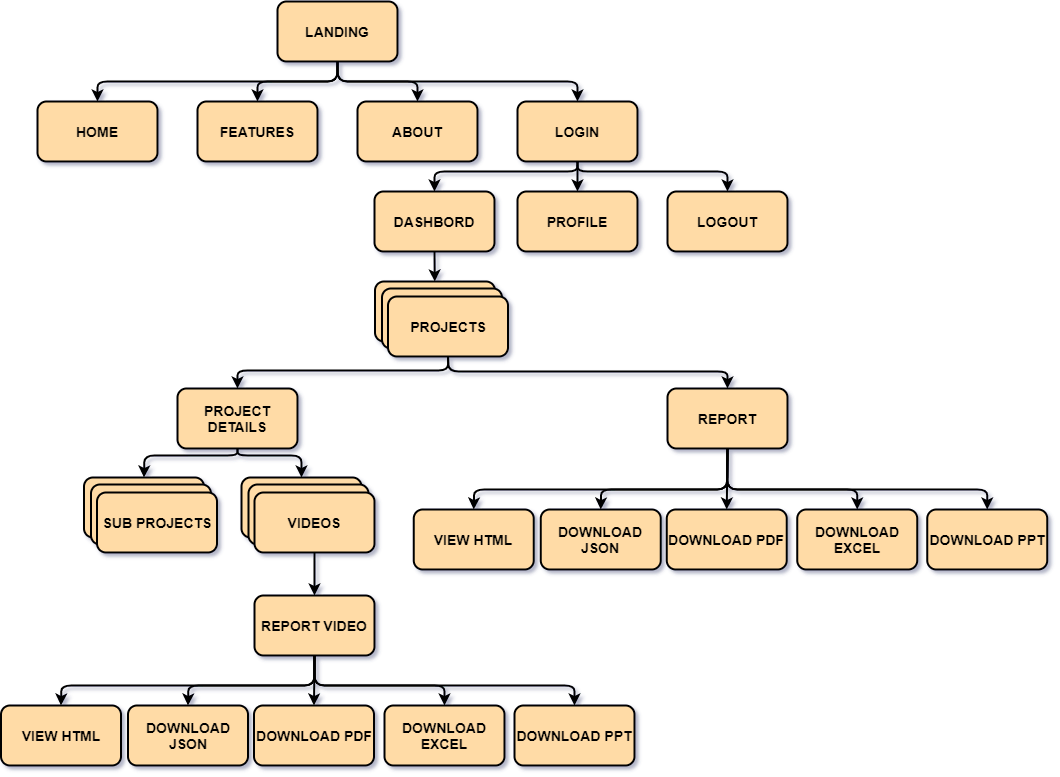
\includegraphics{images/mappa-sito.png}

\section{Storyboard}\label{sec:storyboard}
Gli storyboard sono la rappresentazione di particolari sequenze di navigazione 
del sito, accompagnata da una sintetica descrizione.

\section{Gabbie logiche}\label{sec:gabbie-logiche}
Le gabbie logiche mostrano soltanto menu, spazi e ingombri di massima di 
ciascuna pagina, senza fornire alcuna indicazione precisa sulla grafica.

\section{Prototipo di navigazione}\label{sec:prototipo-navigazione}
È un prototipo piuttosto rudimentale completamente navigabile. Le pagine sono 
costituite dalla sola gabbia logica, in bianco e nere, senza grafica, senza 
contenuti informativi e il <<testo fittizio>> inserito nella gabbia logica.


